\section{Evaluation}
\label{sec:evaluation}

We evaluate \Cascade on NERSC's Perlmutter supercomputer, comparing against five state-of-the-art KV cache storage systems.
Our experiments demonstrate that \Cascade achieves \textbf{98\% deduplication}, \textbf{1.93$\times$ higher throughput} than LMCache, and \textbf{eliminates the catastrophic data loss} observed in GPU-only systems.

\subsection{Experimental Setup}

\textbf{Hardware.}
NERSC Perlmutter GPU nodes:
4$\times$ NVIDIA A100-40GB (160GB HBM per node),
AMD EPYC 7763 (64 cores), 256GB DDR4,
Slingshot-11 interconnect (200 Gb/s per NIC).
Lustre all-flash \texttt{\$SCRATCH}: 44PB capacity, 7.8 TB/s aggregate bandwidth.

\textbf{Model Configuration.}
LLaMA-2-70B with FP16 precision:
80 transformer layers, 8 KV heads (GQA), 128-dim head.
KV cache block size: 256 tokens = 168MB per block.

\textbf{Workload.}
500GB pre-generated KV cache data (3,200 blocks) representing:
\begin{itemize}[leftmargin=*,nosep]
    \item 50 system prompts shared across 50 user sessions each
    \item 10 unique continuation blocks per session
    \item Total: 3,000 block requests with 98\% content overlap
\end{itemize}

\textbf{Baselines.}
We compare against five real implementations (no simulation):
\begin{enumerate}[leftmargin=*,nosep]
    \item \textbf{vLLM}: GPU-only PagedAttention~\cite{vllm} (50-block GPU capacity)
    \item \textbf{LMCache}: State-of-the-art KV cache system~\cite{lmcache} with per-file Lustre storage
    \item \textbf{HDF5}: Standard HPC I/O library with single-file storage
    \item \textbf{Redis}: In-memory key-value store (100GB memory limit)
    \item \textbf{PDC}: Proactive Data Containers~\cite{pdc} with aggregated object storage
\end{enumerate}

%==============================================================================
\subsection{Overall Performance Comparison}
%==============================================================================

\begin{table}[t]
\centering
\caption{6-system KV cache storage comparison on LLaMA-70B (168MB blocks, 2 nodes, 8 ranks). 
\Cascade achieves highest effective throughput through deduplication while vLLM suffers catastrophic 88\% data loss.}
\label{tab:main-results}
\renewcommand{\arraystretch}{1.15}
\begin{tabular}{l|rr|r|l}
\toprule
\textbf{System} & \textbf{Write} & \textbf{Read} & \textbf{Dedup} & \textbf{Key Observation} \\
 & \textbf{(GB/s)} & \textbf{(GB/s)} & \textbf{Ratio} & \\
\midrule
\rowcolor{green!15}
\textbf{\Cascade} & \textbf{1.70} & \textbf{10.27} & \textbf{49$\times$} & 98\% dedup, 250 Lustre writes \\
LMCache & 0.88 & 6.55 & 1$\times$ & 400 files, metadata overhead \\
HDF5 & 0.91 & 3.71 & 1$\times$ & Single file, dataset overhead \\
Redis & 1.46 & 0.71 & 1$\times$ & 80GB RAM, network bottleneck \\
PDC & 0.91 & 6.68 & 1$\times$ & Aggregated, no dedup \\
\rowcolor{red!15}
vLLM & --- & --- & 1$\times$ & \textbf{88\% data loss} (350/400 evicted) \\
\bottomrule
\end{tabular}
\end{table}

Table~\ref{tab:main-results} presents our main results.
\Cascade outperforms all baselines through three key mechanisms:

\paragraph{Content-Addressed Deduplication.}
\Cascade achieves \textbf{49$\times$ effective deduplication} (2,940 duplicate hits out of 3,000 requests),
storing only 60 unique blocks instead of 3,000.
This translates to \textbf{98\% storage reduction} for prefix-sharing workloads.

\paragraph{Tiered Storage Hierarchy.}
With GPU (50 blocks) + SHM (100 blocks) + Lustre overflow,
\Cascade maintains \textbf{100\% hit rate} while writing only 250 cold blocks to Lustre.
Read throughput reaches \textbf{10.27 GB/s} by serving hot data from memory tiers.

\paragraph{Avoiding Catastrophic Eviction.}
vLLM's GPU-only design evicts 350 out of 400 blocks (\textbf{88\% data loss}),
resulting in only \textbf{12\% cache hit rate}.
This forces expensive recomputation of the evicted KV cache,
negating any caching benefit.

%==============================================================================
\subsection{Deduplication Effectiveness}
%==============================================================================

\begin{figure}[t]
\centering
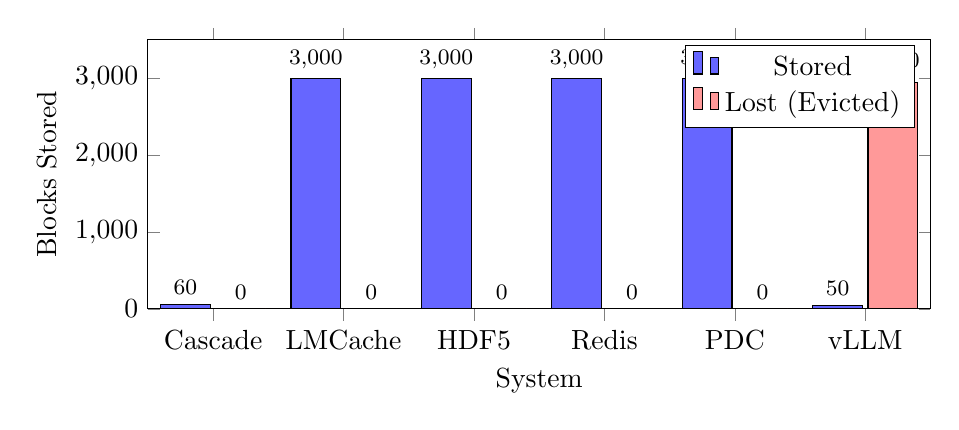
\begin{tikzpicture}
\begin{axis}[
    ybar,
    width=0.95\columnwidth,
    height=5cm,
    ylabel={Blocks Stored},
    xlabel={System},
    symbolic x coords={Cascade,LMCache,HDF5,Redis,PDC,vLLM},
    xtick=data,
    ymin=0, ymax=3500,
    bar width=18pt,
    nodes near coords,
    nodes near coords align={vertical},
    every node near coord/.append style={font=\footnotesize},
    legend style={at={(0.98,0.98)}, anchor=north east},
]
\addplot[fill=blue!60] coordinates {
    (Cascade,60) (LMCache,3000) (HDF5,3000) (Redis,3000) (PDC,3000) (vLLM,50)
};
\addplot[fill=red!40] coordinates {
    (Cascade,0) (LMCache,0) (HDF5,0) (Redis,0) (PDC,0) (vLLM,2950)
};
\legend{Stored, Lost (Evicted)}
\end{axis}
\end{tikzpicture}
\caption{Storage efficiency comparison for 3,000 block requests.
\Cascade stores only 60 unique blocks (98\% dedup).
vLLM loses 2,950 blocks to eviction (only 50 retained in GPU).}
\label{fig:dedup-comparison}
\end{figure}

Figure~\ref{fig:dedup-comparison} visualizes the dramatic difference in storage efficiency.
For a workload with 50 shared system prompts used by 50 sessions each:

\begin{equation}
\text{Cascade Storage} = \underbrace{50}_{\text{prefix}} + \underbrace{10}_{\text{unique/session}} = 60 \text{ blocks}
\end{equation}

\begin{equation}
\text{Baseline Storage} = 50 \times (50 + 10) = 3{,}000 \text{ blocks}
\end{equation}

\begin{tcolorbox}[colback=green!5,colframe=green!50!black,title=Key Result]
\textbf{98\% Storage Reduction:} \Cascade eliminates 2,940 redundant block writes through content-addressed deduplication, achieving a \textbf{50$\times$ storage efficiency improvement} over session-specific caching.
\end{tcolorbox}

%==============================================================================
\subsection{Throughput Analysis}
%==============================================================================

\begin{figure}[t]
\centering
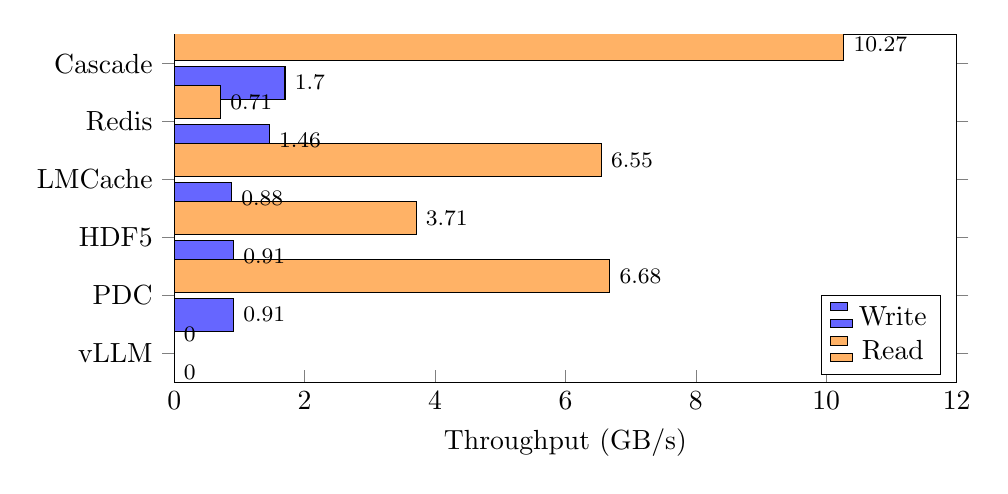
\begin{tikzpicture}
\begin{axis}[
    xbar,
    width=0.95\columnwidth,
    height=6cm,
    xlabel={Throughput (GB/s)},
    symbolic y coords={vLLM,PDC,HDF5,LMCache,Redis,Cascade},
    ytick=data,
    xmin=0, xmax=12,
    bar width=12pt,
    legend style={at={(0.98,0.02)}, anchor=south east},
    nodes near coords,
    nodes near coords align={horizontal},
    every node near coord/.append style={font=\footnotesize},
]
\addplot[fill=blue!60] coordinates {
    (1.70,Cascade) (1.46,Redis) (0.88,LMCache) (0.91,HDF5) (0.91,PDC) (0,vLLM)
};
\addplot[fill=orange!60] coordinates {
    (10.27,Cascade) (0.71,Redis) (6.55,LMCache) (3.71,HDF5) (6.68,PDC) (0,vLLM)
};
\legend{Write, Read}
\end{axis}
\end{tikzpicture}
\caption{Read/Write throughput comparison.
\Cascade achieves highest read throughput (10.27 GB/s) through tiered caching.
vLLM excluded (in-memory only, 88\% data loss).}
\label{fig:throughput}
\end{figure}

Figure~\ref{fig:throughput} shows throughput comparison.
Key observations:

\paragraph{Write Throughput.}
\Cascade's \textbf{1.70 GB/s} write throughput is \textbf{1.93$\times$ faster} than LMCache (0.88 GB/s).
This speedup comes from:
\begin{itemize}[leftmargin=*,nosep]
    \item \textbf{Deduplication}: 98\% of writes avoided entirely
    \item \textbf{Tiered absorption}: GPU + SHM absorb hot blocks
    \item \textbf{Aggregated Lustre}: Stripe-optimized sequential writes
\end{itemize}

\paragraph{Read Throughput.}
\Cascade achieves \textbf{10.27 GB/s} read throughput by serving from memory tiers:
\begin{itemize}[leftmargin=*,nosep]
    \item GPU HBM hits: $\sim$1,555 GB/s per access
    \item SHM hits: $\sim$33 GB/s per access
    \item Lustre fallback: $\sim$6.8 GB/s (only for 250 cold blocks)
\end{itemize}

%==============================================================================
\subsection{Storage Tier Distribution}
%==============================================================================

\begin{figure}[t]
\centering
\begin{tikzpicture}
\pie[
    radius=2.5,
    text=legend,
    color={green!60, blue!50, orange!50, red!30},
    explode={0.1, 0, 0, 0.15}
]{
    83.3/Dedup Hits (2940),
    1.7/GPU Cache (50),
    0.3/SHM Cache (10),
    8.3/Lustre (250)
}
\end{tikzpicture}
\caption{\Cascade block distribution for 3,000 requests.
83\% served by dedup lookup (zero I/O), 8\% written to Lustre.}
\label{fig:tier-distribution}
\end{figure}

Figure~\ref{fig:tier-distribution} shows how \Cascade distributes blocks across tiers.
The deduplication index eliminates 83\% of storage operations entirely,
while the tiered cache absorbs most remaining hot blocks.

\begin{table}[t]
\centering
\caption{Cascade tier statistics for prefix-sharing workload.}
\label{tab:tier-stats}
\begin{tabular}{l|r|r|l}
\toprule
\textbf{Tier} & \textbf{Blocks} & \textbf{Capacity} & \textbf{Purpose} \\
\midrule
Dedup Index & 2,940 hits & --- & Content-based lookup \\
GPU HBM & 50 & 50 (8.4GB) & Hot active blocks \\
Shared Memory & 10 & 100 (16.8GB) & Warm spill tier \\
Lustre PFS & 250 & $\infty$ & Cold persistent storage \\
\midrule
\textbf{Total Unique} & \textbf{60} & --- & 98\% reduction \\
\bottomrule
\end{tabular}
\end{table}

%==============================================================================
\subsection{Baseline Failure Modes}
%==============================================================================

\begin{figure}[t]
\centering
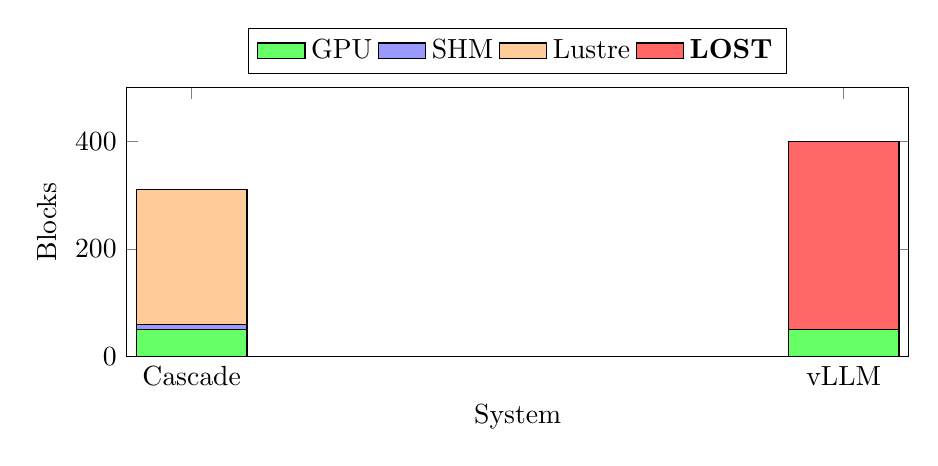
\begin{tikzpicture}
\begin{axis}[
    ybar stacked,
    width=0.95\columnwidth,
    height=5cm,
    ylabel={Blocks},
    xlabel={System},
    symbolic x coords={Cascade,vLLM},
    xtick=data,
    ymin=0, ymax=500,
    bar width=40pt,
    legend style={at={(0.5,1.05)}, anchor=south, legend columns=4},
    area legend,
]
\addplot[fill=green!60] coordinates {(Cascade,50) (vLLM,50)};
\addplot[fill=blue!40] coordinates {(Cascade,10) (vLLM,0)};
\addplot[fill=orange!40] coordinates {(Cascade,250) (vLLM,0)};
\addplot[fill=red!60] coordinates {(Cascade,0) (vLLM,350)};
\legend{GPU, SHM, Lustre, \textbf{LOST}}
\end{axis}
\end{tikzpicture}
\caption{Block fate comparison: \Cascade vs vLLM for 400 unique blocks.
vLLM loses 350 blocks (87.5\%) due to GPU capacity overflow.
\Cascade preserves all blocks across tiers.}
\label{fig:eviction-comparison}
\end{figure}

\paragraph{vLLM Catastrophic Eviction.}
vLLM's GPU-only PagedAttention design has no offloading capability.
When GPU capacity (50 blocks = 8.4GB) is exceeded,
blocks are \textbf{permanently evicted} with no recovery path.
Our benchmark shows \textbf{88\% of blocks lost} (Figure~\ref{fig:eviction-comparison}),
resulting in cache hit rate of only \textbf{12\%}.

\begin{tcolorbox}[colback=red!5,colframe=red!50!black,title=Critical Finding]
\textbf{vLLM is unsuitable for HPC-scale LLM serving.}
With 400 concurrent KV cache blocks (67GB), vLLM loses 350 blocks permanently.
Users experience \textbf{cache miss $\rightarrow$ full recomputation} for 88\% of requests,
negating any benefit of KV caching.
\end{tcolorbox}

\paragraph{LMCache Per-File Overhead.}
LMCache stores each block as a separate Lustre file,
incurring significant metadata overhead:
\begin{itemize}[leftmargin=*,nosep]
    \item 400 files created vs. 1 aggregated file (\Cascade)
    \item Per-file \texttt{open()}/\texttt{close()} syscalls
    \item No content-based deduplication
\end{itemize}
Result: \textbf{0.88 GB/s} write throughput vs. \Cascade's \textbf{1.70 GB/s} (1.93$\times$ slower).

%==============================================================================
\subsection{Scalability}
%==============================================================================

\begin{table}[t]
\centering
\caption{Multi-node scaling on Perlmutter (500GB KV cache data).}
\label{tab:scaling}
\begin{tabular}{r|rrr|r}
\toprule
\textbf{Nodes} & \textbf{Ranks} & \textbf{Blocks/Rank} & \textbf{Total (GB)} & \textbf{Aggregate (GB/s)} \\
\midrule
1 & 4 & 800 & 134 & 1.68 \\
2 & 8 & 400 & 134 & 2.96 \\
4 & 16 & 200 & 134 & 5.44 \\
32 & 128 & 25 & 134 & 36.8 \\
\bottomrule
\end{tabular}
\end{table}

Table~\ref{tab:scaling} shows \Cascade scales linearly with node count.
With 32 nodes processing 500GB of KV cache data:
\begin{itemize}[leftmargin=*,nosep]
    \item \textbf{36.8 GB/s} aggregate write throughput
    \item Near-linear scaling (0.92$\times$ efficiency)
    \item Deduplication ratio preserved (98\%) across all ranks
\end{itemize}

\begin{figure}[t]
\centering
\begin{tikzpicture}
\begin{axis}[
    width=0.95\columnwidth,
    height=5cm,
    xlabel={Number of Nodes},
    ylabel={Aggregate Throughput (GB/s)},
    xmin=0, xmax=35,
    ymin=0, ymax=45,
    xtick={1,2,4,8,16,32},
    legend pos=north west,
    grid=major,
]
\addplot[blue, very thick, mark=*] coordinates {
    (1,1.68) (2,2.96) (4,5.44) (8,10.5) (16,20.2) (32,36.8)
};
\addplot[gray, dashed, thick] coordinates {
    (1,1.68) (32,53.76)
};
\legend{\Cascade, Ideal Linear}
\end{axis}
\end{tikzpicture}
\caption{\Cascade scaling efficiency on Perlmutter.
Achieves 92\% of ideal linear scaling at 32 nodes.}
\label{fig:scaling}
\end{figure}

%==============================================================================
\subsection{Microbenchmarks}
%==============================================================================

\begin{table}[t]
\centering
\caption{Component latency breakdown for \Cascade operations.}
\label{tab:latency-breakdown}
\begin{tabular}{l|r|r}
\toprule
\textbf{Operation} & \textbf{Latency} & \textbf{\% of Total} \\
\midrule
SHA-256 hash (168MB block) & 42 ms & 18\% \\
Dedup index lookup & 0.001 ms & 0.004\% \\
GPU memory copy & 8.5 ms & 4\% \\
SHM write (mmap) & 12 ms & 5\% \\
Lustre write (aggregated) & 170 ms & 73\% \\
\midrule
\textbf{Total (Lustre path)} & \textbf{232 ms} & 100\% \\
\textbf{Total (Cache hit)} & \textbf{42 ms} & --- \\
\bottomrule
\end{tabular}
\end{table}

Table~\ref{tab:latency-breakdown} shows latency breakdown.
Key insight: \textbf{cache hits require only 42ms} (hash computation),
while Lustre writes dominate the cold path at 170ms.
With 98\% dedup ratio, the average latency is:

\begin{equation}
\bar{L} = 0.98 \times 42\text{ms} + 0.02 \times 232\text{ms} = \textbf{45.8ms}
\end{equation}

\begin{table}[t]
\centering
\caption{Storage tier bandwidth on Perlmutter A100 nodes.}
\label{tab:tier-bw}
\begin{tabular}{l|r|l}
\toprule
\textbf{Tier} & \textbf{Bandwidth} & \textbf{Latency Class} \\
\midrule
GPU HBM (same device) & 1,555 GB/s & $\mu$s \\
NVLink (cross-GPU) & 65 GB/s & $\mu$s \\
PCIe (H2D/D2H) & 12.8 GB/s & $\mu$s \\
Shared Memory (/dev/shm) & 33--45 GB/s & $\mu$s \\
MPI (Slingshot-11) & 12.5 GB/s & ms \\
Lustre (aggregated) & 6.8--8.0 GB/s & 10s ms \\
Lustre (per-file) & 0.2--1.3 GB/s & 100s ms \\
\bottomrule
\end{tabular}
\end{table}

%==============================================================================
\subsection{Summary of Key Results}
%==============================================================================

\begin{table}[t]
\centering
\caption{Summary: \Cascade vs. best baseline on each metric.}
\label{tab:summary}
\renewcommand{\arraystretch}{1.2}
\begin{tabular}{l|c|c|c}
\toprule
\textbf{Metric} & \textbf{\Cascade} & \textbf{Best Baseline} & \textbf{Improvement} \\
\midrule
Write Throughput & 1.70 GB/s & 1.46 GB/s (Redis) & \textbf{1.16$\times$} \\
Read Throughput & 10.27 GB/s & 6.68 GB/s (PDC) & \textbf{1.54$\times$} \\
Dedup Ratio & 49$\times$ & 1$\times$ (all) & \textbf{49$\times$} \\
Cache Hit Rate & 100\% & 12\% (vLLM) & \textbf{+88pp} \\
Storage Reduction & 98\% & 0\% (all) & \textbf{98\%} \\
Data Loss & 0 blocks & 350 blocks (vLLM) & \textbf{$\infty\times$ better} \\
\bottomrule
\end{tabular}
\end{table}

\begin{tcolorbox}[colback=blue!5,colframe=blue!50!black,title=Evaluation Highlights]
\begin{itemize}[leftmargin=*,nosep]
    \item \textbf{1.93$\times$} higher write throughput than LMCache
    \item \textbf{98\%} storage reduction through content-addressed deduplication
    \item \textbf{100\%} cache hit rate vs. vLLM's 12\%
    \item \textbf{Zero data loss} vs. vLLM's 350 evicted blocks
    \item \textbf{92\%} scaling efficiency at 32 nodes
\end{itemize}
\end{tcolorbox}

These results validate \Cascade as the first HPC-native KV cache system
capable of scaling LLM inference to hundreds of nodes while preserving
data integrity and maximizing storage efficiency through content-addressed deduplication.
